\documentclass[aspectratio=169,t,xcolor=table]{beamer}
\usepackage[utf8]{inputenc}
\usepackage[english]{babel} %Con este paquete se establece el idioma español

\usepackage{svg}
\usepackage{booktabs} 
\usepackage{subcaption}
\usepackage{amsmath,etoolbox}
\usepackage{threeparttable}
\usepackage{multirow}
\usepackage{array}
% \usepackage{subfigure}
\usepackage{algorithm}
\usepackage{algpseudocode}
\usepackage{tabularx}
\usepackage{makecell}
\usepackage{graphicx}
\usepackage{framed}
\definecolor{shadecolor}{gray}{0.9}
\usepackage{tikz,lipsum,lmodern}
\usepackage[most]{tcolorbox}
\usepackage{highlight}
% \captionsetup[table]{font=tiny,skip=50pt}
% \captionsetup[figure]{font=tiny,skip=-50pt}

\usepackage{lipsum}
\usepackage[absolute,overlay]{textpos}

\usetheme{Ufg}
\setbeamercolor{framesource}{fg=gray}
\setbeamerfont{framesource}{size=\tiny}


%-------------------------------------theorems--------------
% \newtheorem{conj}{Conjetura}
% \newtheorem{defi}{Definição}
% \newtheorem{teo}{Teorema}
% \newtheorem{lema}{Lema}
% \newtheorem{prop}{Proposição}
% \newtheorem{cor}{Corolário}
% \newtheorem{ex}{Exemplo}
% \newtheorem{exer}{Exercício}

% \setbeamertemplate{theorems}[numbered]
% \setbeamertemplate{caption}[numbered]

% ---------------------Cite images----------------------------%
\newcommand{\source}[1]{\begin{textblock*}{5.4cm}(9cm,8.4cm)
    \begin{beamercolorbox}[ht=0.5cm,right]{framesource}
        \usebeamerfont{framesource}\usebeamercolor[fg]{framesource} Source: {#1}
    \end{beamercolorbox}
\end{textblock*}}


%-------------------------------------------------------------%
%----------------------- Primary Definitions -----------------%

% This command set the default Color, is also possible to choose a custom color
\setPrimaryColor{EHUBlue} 

% First one is logo in title slide (we recommend use a horizontal image), and second one is the logo used in the remaining slides (we recommend use a square image)
\setLogos{lib/logos/EHU_logo.png}{lib/logos/EHU_logo.png} 

\title{Module 1: Introduction to Hardware Acceleration}
\subtitle{Hardware Acceleration for AI}
\author{Your Name}
\institute{Your Institution}
\date{\today}

\begin{document}

% Title slide
\begin{frame}
    \titlepage
\end{frame}

% Main introduction slide
\begin{frame}
    \setLayout{horizontal}  % Using the template's horizontal layout
    \frametitle{From room-sized computers to AI in your pocket}
    \vspace{-0.3cm}%
    \begin{block}{The Evolution of Hardware for Artificial Intelligence}
        From the first electronic computers to modern AI accelerators
    \end{block}
    \vspace{5 cm}
    \begin{tikzpicture}[overlay,remember picture]
        % Computer evolution illustration
        \begin{scope}[shift={(current page.center)}, yshift=-2cm]
            % Timeline base
            \draw[MUBlue, thick] (-6,0) -- (6,0);
            \foreach \x in {-6,-4,-2,0,2,4}
                \draw[MUBlue, thick] (\x,-0.1) -- (\x,0.1);
            
            % ENIAC-style computer (far left)
            \draw[fill=MUBlue!10, draw=MUBlue] (-5.5,0.5) rectangle (-4.5,2.5);
            \foreach \x in {-5.3,-5,-4.7}
                \foreach \y in {0.7,1.1,1.5,1.9,2.3}
                    \fill[MUBlue!40] (\x,\y) circle (0.1);
            
            % Desktop computer
            \draw[fill=MUBlue!10, draw=MUBlue] (-3,0.5) rectangle (-2,2);
            \draw[fill=MUBlue!5, draw=MUBlue] (-2.8,0.7) rectangle (-2.2,1.8);
            \draw[fill=MUBlue!10, draw=MUBlue] (-2.7,0.3) rectangle (-2.3,0.5);
            
            % Workstation/Server
            \draw[fill=MUBlue!10, draw=MUBlue] (-0.5,0.5) rectangle (0.5,1.5);
            \foreach \y in {0.7,1,1.3}
                \draw[MUBlue] (-0.3,\y) -- (0.3,\y);
            
            % Laptop
            \path[fill=MUBlue!10, draw=MUBlue] (2,0.5) -- (3,0.5) -- (3,1.5) -- (2,1.5) -- cycle;
            \path[fill=MUBlue!5, draw=MUBlue] (2,0.3) -- (3,0.3) -- (3,0.5) -- (2,0.5) -- cycle;
            
            % Smartphone
            \draw[fill=MUBlue!10, draw=MUBlue, rounded corners=2pt] (4.5,0.5) rectangle (5,2);
            \draw[fill=MUBlue!5, draw=MUBlue, rounded corners=1pt] (4.6,0.6) rectangle (4.9,1.8);
            \draw[fill=MUBlue] (4.7,0.7) circle (0.05);
            
            % Year labels
            \node[below] at (-6,0) {\small 1945};
            \node[below] at (-4,0) {\small 1970};
            \node[below] at (-2,0) {\small 1990};
            \node[below] at (0,0) {\small 2000};
            \node[below] at (2,0) {\small 2010};
            \node[below] at (4,0) {\small 2020};
            
            % Device labels
            \node[above, text width=2cm, align=center] at (-5,2.8) {\small ENIAC};
            \node[above, text width=2cm, align=center] at (-2.5,2.3) {\small Personal\\Computer};
            \node[above, text width=2cm, align=center] at (0,1.8) {\small GPU\\Servers};
            \node[above, text width=2cm, align=center] at (2.5,1.8) {\small AI\\Workstations};
            \node[above, text width=2cm, align=center] at (4.75,2.3) {\small Edge\\Devices};
        \end{scope}
    \end{tikzpicture}

    \vspace{3cm}  % Add space after the tikz picture
    

    \note{
    Teaching points:
    \begin{itemize}
        \item ENIAC filled a room and had less power than a modern calculator
        \item Modern phones have more AI power than early supercomputers
        \item Discussion prompt: Ask students about their first computer
    \end{itemize}
    
    Time management:
    \begin{itemize}
        \item Spend 5 minutes on introduction
        \item Allow 2-3 minutes for student responses
    \end{itemize}
}
\end{frame}
\begin{frame}

\begin{figure}
    \centering
    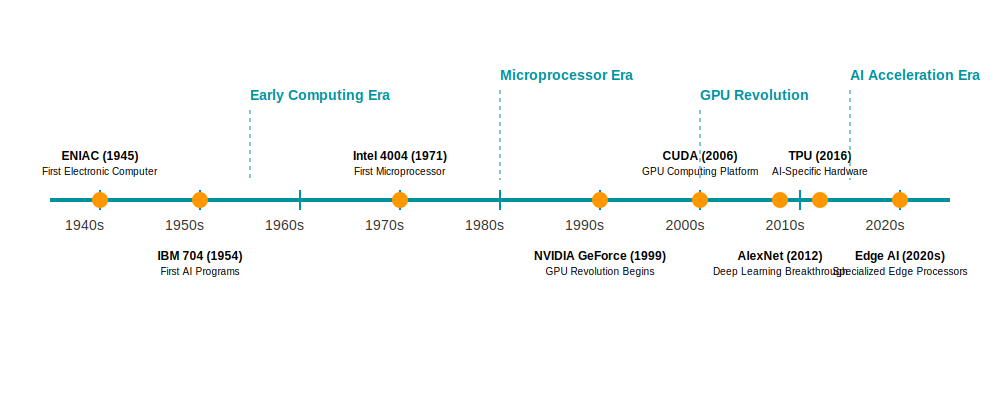
\includegraphics[width=\textwidth]{figs/ai-hardware-timeline}  % don't include the .pdf extension
    \caption{Computing Evolution Timeline}
\end{figure}
\end{frame}
\begin{frame}
    \setLayout{horizontal}
    \frametitle{Early Computing and AI (1940s-1970s)}
    
    \begin{columns}[t] % 't' for top alignment
        \begin{column}{0.58\textwidth}
            \begin{block}{First Steps in Computing}
                \small % Reduce text size
                \begin{itemize}\setlength{\itemsep}{0pt} % Reduce item spacing
                    \item ENIAC (1945)
                    \begin{itemize}\setlength{\itemsep}{0pt}
                        \item First general-purpose electronic computer
                        \item Basic numerical calculations
                        \item 17,468 vacuum tubes
                    \end{itemize}
                    \item Early mainframe systems
                    \begin{itemize}\setlength{\itemsep}{0pt}
                        \item IBM 704 (1954) - First AI programs
                        \item PDP-11 (1970) - Minicomputer revolution
                    \end{itemize}
                \end{itemize}
            \end{block}
            
            \vspace{-0.2cm} % Reduce space between blocks
            
        \end{column}
        
        \begin{column}{0.38\textwidth}
            \begin{alertblock}{Key Challenges}
                \small % Reduce text size
                \begin{itemize}\setlength{\itemsep}{0pt} % Reduce item spacing
                    \item Sequential processing limitations
                    \item Memory constraints
                    \item Enormous size and cost
                    \item High maintenance requirements
                \end{itemize}
            \end{alertblock}
            \begin{exampleblock}{Notable Achievements}
                \small % Reduce text size
                \begin{itemize}\setlength{\itemsep}{0pt} % Reduce item spacing
                    \item Logic Theorist (1956)
                    \item General Problem Solver
                    \item First Natural Language Processing
                \end{itemize}
            \end{exampleblock}
            
        \end{column}
    \end{columns}
\end{frame}

\begin{frame}
    \setLayout{horizontal}
    \frametitle{Early Computing: ENIAC and Evolution}
    
    \begin{columns}[t]
        % Left column for ENIAC photo
        \begin{column}{0.45\textwidth}
            \begin{block}{ENIAC (1945)}
                \centering
                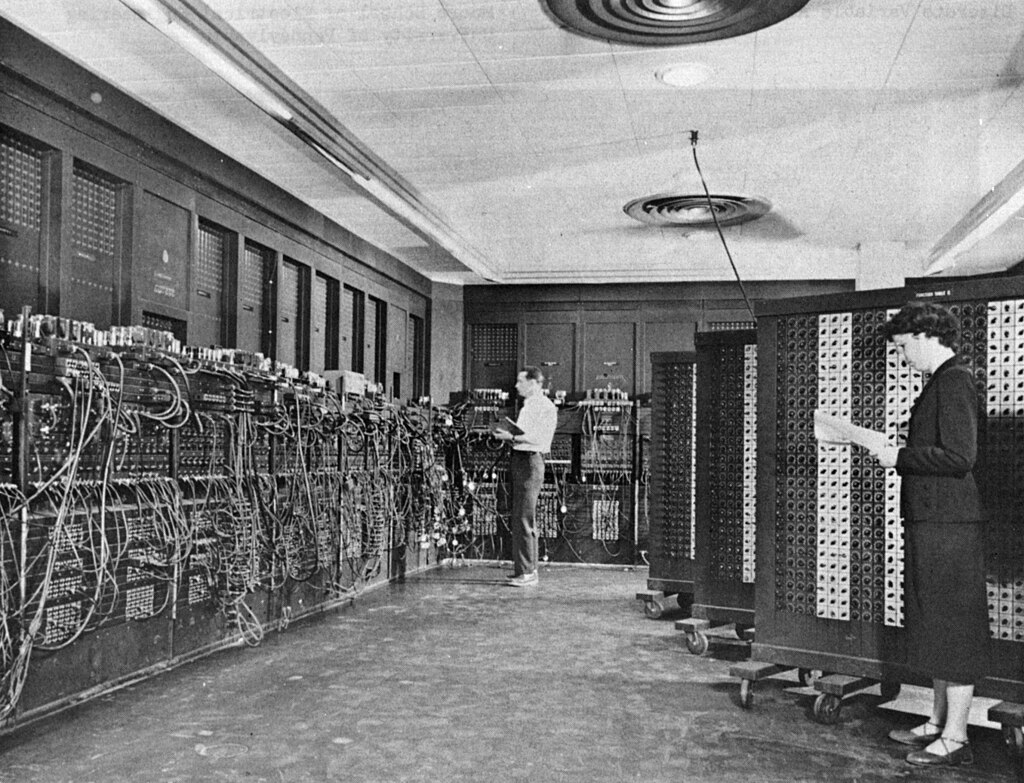
\includegraphics[width=\textwidth]{figs/eniac.jpg}
                \small{First general-purpose electronic computer}
            \end{block}
            
            \vspace{-0.2cm}
            
        \end{column}
        
        % Right column for timeline
        \begin{column}{0.5\textwidth}
            \begin{alertblock}{Key Facts}
                \small
                \begin{itemize}\setlength{\itemsep}{0pt}
                    \item Weight: 30 tons
                    \item Space: 167 $m^2$ 
                    \item Power: 150kW
                    \item Cost: \$6M (today's value)
                \end{itemize}
            \end{alertblock}
            
        \end{column}
    \end{columns}
\end{frame}

\begin{frame}{Evolution of computing power}.
    \vspace{-2cm}
    \begin{block}{AI Hardware Evolution (1946-Present)}
    \centering
    \begin{tikzpicture}[scale=0.85]
        % Using wider rectangle for 16:9 aspect ratio
        \draw[white,fill=white!98] (0,0) rectangle (12,6);
        
        % Axes
        \draw[->,thick] (1,0.5) -- (1,5.5) node[above] {\small Computing Power (TFLOPS)};
        \draw[->,thick] (1,0.5) -- (11,0.5) node[right] {\small Size (cm²)};
        
        % Grid and labels
        % Y-axis labels (TFLOPS - using log scale)
        \foreach \y/\flops in {1/0.001, 2/0.01, 3/0.1, 4/1, 5/10} {
            \draw[gray!20] (1,\y) -- (11,\y);
            \node[left,font=\tiny] at (0.9,\y) {\flops};
        }
        
        % X-axis labels (Size in cm²)
        \foreach \x/\size in {2/10, 4/100, 6/1K, 8/10K, 10/100K} {
            \draw[gray!20] (\x,0.5) -- (\x,5);
            \node[below,font=\tiny] at (\x,0.4) {\size};
        }
            
        % Historical to Modern Systems (positions adjusted for accuracy)
        % Early Era (Large size, low compute)
        \node[circle,fill=MUBlue,inner sep=1.5pt] (eniac) at (9.5,1) {};
        \node[font=\tiny] at (9.5,0.7) {ENIAC (1946)};
        
        \node[circle,fill=MUBlue,inner sep=1.5pt] (ibm704) at (8.5,1.5) {};
        \node[font=\tiny] at (8.5,1.2) {IBM 704 (1954)};
        
        % Mid Era
        \node[circle,fill=MUBlue,inner sep=1.5pt] (cm2) at (7,2.2) {};
        \node[font=\tiny] at (7,1.9) {CM-2 (1987)};
        
        \node[circle,fill=MUBlue,inner sep=1.5pt] (gpu) at (5,3) {};
        \node[font=\tiny] at (5,2.7) {First GPU AI (2006)};
        
        % Modern Era (Smaller size, high compute)
        \node[circle,fill=MUBlue,inner sep=1.5pt] (tpu) at (3.5,4) {};
        \node[font=\tiny] at (3.5,3.7) {TPU v1 (2016)};
        
        \node[circle,fill=MUBlue,inner sep=1.5pt] (a100) at (4,4.5) {};
        \node[font=\tiny] at (4,4.2) {A100 (2020)};
        
        % Edge Devices (Very small size)
        \node[circle,fill=MUBlue,inner sep=1.5pt] (jetson) at (2,3.5) {};
        \node[font=\tiny] at (2,3.2) {Jetson Nano (2019)};
        
        \node[circle,fill=MUBlue,inner sep=1.5pt] (coral) at (1.8,3.2) {};
        \node[font=\tiny] at (1.8,2.9) {Coral Edge (2019)};
        
        % Connect points
        \draw[MUBlue,dashed] (eniac) -- (ibm704) -- (cm2) -- 
                            (gpu) -- (tpu) -- (a100);
        \draw[MUBlue,dashed] (gpu) -- (jetson);
        \draw[MUBlue,dashed] (gpu) -- (coral);
        
        % Era labels with clearer positioning
        \node[font=\tiny,color=MUBlue] at (9,4) {Mainframe Era};
        \node[font=\tiny,color=MUBlue] at (6,4) {GPU Revolution};
        \node[font=\tiny,color=MUBlue] at (3,4.8) {AI Accelerators};
        \node[font=\tiny,color=MUBlue] at (2,2.5) {Edge AI};
        
        % Legend
        \node[font=\tiny,align=left] at (6.5,5.2) {
            \begin{tabular}{l}
            Size indicates physical footprint\\
            Performance in TeraFLOPS (TFLOPS)\\
            K = thousands, Edge devices $<$ 100cm²
            \end{tabular}
        };
    \end{tikzpicture}
\end{block}
\end{frame}

\begin{frame}
    \setLayout{horizontal}
    \frametitle{Early AI: Logic Theorist and Beyond}
    
    \begin{columns}[t]
        % Left column for Logic Theorist
        \begin{column}{0.48\textwidth}
            \begin{block}{Logic Theorist (1956)}
                \centering
                \begin{tikzpicture}[scale=0.8]
                    % Simple representation of logical reasoning
                    \node[draw,circle,fill=MUBlue!10] (A) at (0,2) {A};
                    \node[draw,circle,fill=MUBlue!10] (B) at (2,2) {B};
                    \node[draw,circle,fill=MUBlue!10] (C) at (1,0) {C};
                    
                    \draw[->,thick,MUBlue] (A) -- (B) node[midway,above] {IF};
                    \draw[->,thick,MUBlue] (B) -- (C) node[midway,right] {THEN};
                    \draw[->,thick,MUBlue] (A) to[bend right] (C) node[midway,left] {THEREFORE};
                \end{tikzpicture}
            \end{block}
            
            \begin{alertblock}{Achievements}
                \small
                \begin{itemize}\setlength{\itemsep}{0pt}
                    \item First AI program in history
                    \item Proved 38 of 52 theorems from Principia Mathematica
                    \item Demonstrated automated reasoning
                \end{itemize}
            \end{alertblock}
        \end{column}
        
        % Right column for impact
        \begin{column}{0.48\textwidth}
            \begin{block}{Historical Impact}
                \small
                \begin{itemize}\setlength{\itemsep}{0pt}
                    \item Proved machines could perform reasoning
                    \item Led to development of:
                    \begin{itemize}\setlength{\itemsep}{0pt}
                        \item Automated theorem provers
                        \item Expert systems
                        \item Modern AI reasoning systems
                    \end{itemize}
                    \item Created by Allen Newell and Herbert Simon
                \end{itemize}
            \end{block}
            
            \begin{exampleblock}{Legacy}
                \small
                Established the foundation for:
                \begin{itemize}\setlength{\itemsep}{0pt}
                    \item Symbolic AI
                    \item Automated problem solving
                    \item Modern theorem provers
                \end{itemize}
            \end{exampleblock}
        \end{column}
    \end{columns}
\end{frame}

\note{
    Frame 1 teaching points:
    \begin{itemize}
        \item Emphasize the physical scale of ENIAC
        \item Compare power consumption to modern devices
        \item Discuss the trend of miniaturization
    \end{itemize}
    
    Frame 2 teaching points:
    \begin{itemize}
        \item Explain the significance of automated theorem proving
        \item Connect to modern AI reasoning systems
        \item Discuss why Logic Theorist was revolutionary
    \end{itemize}
}

\end{document}